\documentclass[sigconf]{acmart}

\usepackage{booktabs} % For formal tables
\usepackage{algorithm,algorithmicx}
\usepackage{tabularx}
%\usepackage{amsmath}
%\usepackage{wasysym}
\usepackage{amssymb}
\usepackage{amsthm}
% Copyright
%\setcopyright{none}
%\setcopyright{acmcopyright}
%\setcopyright{acmlicensed}
\setcopyright{rightsretained}
%\setcopyright{usgov}
%\setcopyright{usgovmixed}
%\setcopyright{cagov}
%\setcopyright{cagovmixed}
\newtheorem{defn}{Definition}[section] % definition objects
\newtheorem{thm}{Theorem}[section] % theorem objects
% DOI
\acmDOI{10.1145/nnnnnnn.nnnnnnn}

% ISBN
\acmISBN{978-x-xxxx-xxxx-x/YY/MM}

%Conference
\acmConference[GECCO '18]{the Genetic and Evolutionary Computation
Conference 2018}{July 15--19, 2018}{Kyoto, Japan}
\acmYear{2018}
\copyrightyear{2018}

\acmPrice{15.00}

\acmSubmissionID{123-A12-B3}

\begin{document}
\title{An analysis of $\epsilon$-lexicase selection for large-scale many-objective optimization}
%\titlenote{Produces the permission block, and copyright information}
%\subtitle{Extended Abstract}
%\subtitlenote{The full version of the author's guide is available as
%  \texttt{acmart.pdf} document}

\author{Anonymous}
%\author{William La Cava}
%%\authornote{Dr.~Trovato insisted his name be first.}
%%\orcid{1234-5678-9012}
%\affiliation{%
%  \institution{University of Pennsylvania}
%  \streetaddress{3700 Hamilton Walk}
%  \city{Philadelphia} 
%  \state{PA} 
%  \postcode{19143}
%}
%\email{lacava@upenn.edu}
%
%\author{Jason H. Moore}
%%\authornote{The secretary disavows any knowledge of this author's actions.}
%\affiliation{%
%  \institution{University of Pennsylvania}
%  \streetaddress{3700 Hamilton Walk}
%  \city{Philadelphia} 
%  \state{PA} 
%  \postcode{19143}
%}
%\email{moore@upenn.edu}

% The default list of authors is too long for headers.
%\renewcommand{\shortauthors}{La Cava and Moore}

\begin{abstract}
In this paper we adapt $\epsilon$-lexicase selection, a parent selection strategy designed for 
genetic programming, to solve many-objective optimization problems. $\epsilon$-lexicase
selection has been shown to perform well in regression due to its use of full program semantics for 
conducting selection. A recent theoretical analysis showed that this selection 
strategy preserves individuals located near the boundaries of the Pareto front in semantic 
space. We hypothesize that this strategy of biasing search to extreme positions in objective space 
may be beneficial for many-objective optimization as the number of objectives increases. Here, we replace program 
semantics with objective fitness to define $\epsilon$-lexicase selection for many-objective optimization. We provide a detailed example $\epsilon$-lexicase selection on a 3 objective problem to illustrate its behavior. We then compare 
this method to multi-objective optimization methods from literature on problems ranging from 3 to 
100 objectives. We find that $\epsilon$-lexicase selection outperforms state-of-the-art optimization 
algorithms in terms of convergence to the Pareto front, spread of solutions, and CPU time for problems with more than 3 objectives.   
\end{abstract}

%
% The code below should be generated by the tool at
% http://dl.acm.org/ccs.cfm
% Please copy and paste the code instead of the example below. 
%
%\begin{CCSXML}
%<ccs2012>
% <concept>
%  <concept_id>10010520.10010553.10010562</concept_id>
%  <concept_desc>Computer systems organization~Embedded systems</concept_desc>
%  <concept_significance>500</concept_significance>
% </concept>
% <concept>
%  <concept_id>10010520.10010575.10010755</concept_id>
%  <concept_desc>Computer systems organization~Redundancy</concept_desc>
%  <concept_significance>300</concept_significance>
% </concept>
% <concept>
%  <concept_id>10010520.10010553.10010554</concept_id>
%  <concept_desc>Computer systems organization~Robotics</concept_desc>
%  <concept_significance>100</concept_significance>
% </concept>
% <concept>
%  <concept_id>10003033.10003083.10003095</concept_id>
%  <concept_desc>Networks~Network reliability</concept_desc>
%  <concept_significance>100</concept_significance>
% </concept>
%</ccs2012>  
%\end{CCSXML}

%\ccsdesc[500]{Computer systems organization~Embedded systems}
%\ccsdesc[300]{Computer systems organization~Redundancy}
%\ccsdesc{Computer systems organization~Robotics}
%\ccsdesc[100]{Networks~Network reliability}


\keywords{many-objective optimization, selection}


\maketitle

\section{Introduction}

The multi-objective optimization (MO) community is increasingly interested in algorithms that can scale
to large numbers of objectives. Typically the name ``many"-objective optimization (MaO) is used to
describe cases in which there are four or more competing objectives.  Dealing with
large numbers of objectives changes the nature of the search space~\cite{farina_optimal_2002,ishibuchi_evolutionary_2008} and as a result, different types of algorithms perform well~\cite{chand_evolutionary_2015}. As research has progressed, studies
have analyzed the ability of evolutionary multi-objective optimization (EMO) algorithms to find or
appapproximate Pareto-optimal solution sets for problems with up to 6~\cite{wagner_pareto-_2007}, 50~\cite{bader_hype:_2011}, and more recently, 100 objectives~\cite{li_empirical_2017}. 

At the same time that EMO research has moved to larger sets of objectives, the genetic algorithm (GA) and genetic programming (GP) communities have shown strong interest in the so-called ``multi-objectivization" of single-objective problems~\cite{knowles_reducing_2001}. In GP, the idea of restructuring search drivers around program semantics, defined as the outputs or behavior of a GP program, has gained traction~\cite{liskowski_comparison_2015}. Rather than aggregating performance across
training instances, semantic methods can re-define the problem as a set of smaller objectives
for driving search. Methods to discover search objectives by clustering~\cite{krawiec_automatic_2015} and
by matrix factorization~\cite{liskowski_discovery_2017} have been proposed that analyze population semantics, extract
sub-problems in the search space, and use mult-objective selection methods according to these
sub-problems. Finally, lexicase selection~\cite{spector_assessment_2012}, a version of which is studied here, uses program semantics to
filter the population via randomized orders of training cases at each selection event. By doing
so it is able to adapt selection pressure to subsets of training cases that are harder to solve. 

A variant of lexicase selection known as $\epsilon$-lexicase selection was introduced to apply
lexicase selection to continuous error spaces for symbolic regression~\cite{la_cava_epsilon-lexicase_2016}. A recent theoretical analysis 
 considered $\epsilon$-lexicase selection through a multi-objective
lens~\cite{la_cava_epsilon-lexicase_2017}. It showed that $\epsilon$-lexicase selects individuals located near boundaries of the Pareto
set defined by the population's error vectors. In this sense, $\epsilon$-lexicase selection 
demonstrated an instance of a multi-objective treatment of regression with promising results. 

In this paper, we seek to evaluate the performance of $\epsilon$-lexicase selection as a
many-objective optimization algorithm. In \S\ref{s:methods}, we describe $\epsilon$-lexicase 
selection and summarize recent theoretical results related to EMO. We then illustrate the 
probabilities of selection as a function of Pareto front location on a three objective problem. In 
\S\ref{s:exp}, we describe our experimental study, which consists of a comparison of three EMO 
methods on the scalable DTLZ problems with up to 100 objectives. The results are presented in 
\S\ref{s:res} and are discussed in \S\ref{s:con} with suggestions for future research directions. 

\section{Methods}\label{s:methods}
We first define $\epsilon$-lexicse selection for EMO problem. In EMO, we wish to optimize a set of
solutions that approximate the Pareto-optimal set. We have the $d$-dimensional decision
space $X \subset \mathbb{R}^d$, the objective space $Z \in \mathbb{R}^m$ with $m$ objectives, and a vector of functions
$\mathcal{F} = (f_1, f_2, \dots, f_m)$ that each map the decision space to real values, i.e. 
$f_i : X \rightarrow \mathbb{R}$. The optimization problem can be formulated as 

\begin{equation}
    \min \mathcal{F}(x) =   (f_1(x), f_2(x), \dots, f_m(x)) \; , \; x \in X   
\end{equation}

In EMO, we seek to approximate the Pareto-optimal set with a population of solutions of size $N$, denoted as 
$\mathcal{N} = \{x^{(i)}\}_{i=1}^N$, where $x^{(i)} = (x_1,\dots,x_d)$ is a vector of $d$ decision variables.
Optimal solutions are those that are non-dominated. Solution $x$ {\it dominates} solution $x'$  if $f(x)
\leq f(x')$ for all $f \in \mathcal{F}$ and there exists at least one $f \in \mathcal{F}$ for which $f(x) < f(x')$. In
addition to dominance, the set of solutions in $\mathcal{N}$ should characterize the Pareto-optimal
set well, meaning they should 1) cover as much of the Pareto-optimal set as possible and 2) cover it as
evently as possible. In our experiments, we use metrics that consider uniformity as well as
convergence. 

\subsection{$\epsilon$-lexicase selection}

We define the $\epsilon$-Lexicase selection algorithm for EMO in Algorithm~\ref{alg}. Each parent
selection begins with the entire population in the selection pool. A random ``case", i.e. objective, is drawn from the
objectives. For this case, each individual is checked: if it is not within $\epsilon$ of the best
objective value in the current selection pool, it is removed from selection. Selection continues to
consider subsequent cases until the objectives are exhausted or the selection pool is reduced
to one individual. If the former happens first, a random individual from the selection pool is
chosen. 

The version of $\epsilon$-lexicase selection we consider here is known as ``semi-dynamic"
$\epsilon$-lexicase selection~\cite{la_cava_epsilon-lexicase_2017}. In this version, $\epsilon$ is 
defined automatically using a population distribution statistic. Let $\mathbf{f}_i$ be the values
for objective $i$ across the population; i.e., 

\begin{equation}
    \mathbf{f}_i &= \{f_i(x) \; \forall x \in \mathcal{N}\} \label{eq:bf}
\end{equation}

We want $\epsilon$ to relate to the difficulty of objective $i$, often estimated using variance. To
improve robustness to outliers, $\epsilon$-lexicase selection uses the median absolute deviation as follows:

\begin{align}
    \lambda(\mathbf{f}) &= \text{median}(| \mathbf{f} - \text{median}(\mathbf{f})|) \label{eq:mad}
    \\
 \epsilon_i &= \lambda(\mathbf{f}_i ) \label{eq:ep} 
\end{align}

As shown in Algorithm~\ref{alg}, Eqns.~\ref{eq:bf}-\ref{eq:ep} are used to determine the cut-off for 
filtering out candidate solutions during selection. $\epsilon$ is calculated only once for each objective
each generation. 
 
 

\begin{algorithm}
    \caption{{\bf : $\epsilon$-Lexicase Selection} applied to individuals $x \in \mathcal{N}$ with
objective values $f_i(x)$,  $f_i \in \mathcal{F}$.}\label{alg}
\noindent{\small
\begin{tabularx}{\columnwidth}{lX} 
    \texttt{Selection}($\mathcal{N,F}$) 	:						&	\\
    \hspace{1em} $\mathcal{P} \leftarrow \emptyset$ & $\lozenge$ parents \\
    \hspace{1em}\textbf{for} $f_i \in \mathcal{F}$: & $\lozenge$ get $\epsilon$ for each $f_i$\\
    \hspace{1em}\hspace{1em}	$\epsilon_i \leftarrow \lambda$($\mathbf{f}_i$) 	&\\
\hspace{1em} \textbf{do} \text{N} \textbf{times}: &\\
\hspace{1em}  \hspace{1em} $\mathcal{P} \leftarrow \mathcal{P} \; \cup \; $\texttt{GetParent}($\mathcal{N,F},\epsilon$) & $\lozenge$ add selection to $\mathcal{P}$ \\
\\
\texttt{GetParent}($\mathcal{N,F},\epsilon$) 	:						&	\\
\hspace{1em}	$\mathcal{F}' \leftarrow \mathcal{F}$	& $\lozenge$	objectives\\
\hspace{1em}	$S \leftarrow \mathcal{N}$	& $\lozenge$	 selection pool\\
\hspace{1em}	\textbf{while} $|\mathcal{F}'| >0$ \textbf{and} $|\mathcal{S}|>1$:						&	\\
\hspace{1em}\hspace{1em}	$f_i$ $\leftarrow$ random choice from $\mathcal{F'}$ & $\lozenge$ pick random $f_i$ \\
\hspace{1em}\hspace{1em}	$f_i^*$ $\leftarrow$ min $f_i(x)$ \textbf{for} $x \in \mathcal{S}$ 	&$\lozenge$ best score on $f_i$ in pool\\
\hspace{1em}\hspace{1em}	\textbf{for} $x \in \mathcal{S}$: 	&$\lozenge$ filter pool\\
\hspace{1em}\hspace{1em}\hspace{1em}	 \textbf{if} $f_i(x)$ $> f_i^*+\epsilon_{m}$ \textbf{then}&\\
\hspace{1em}\hspace{1em}\hspace{1em}\hspace{1em} $\mathcal{S} \leftarrow \mathcal{S} \setminus \{x\}$	 & \\
\hspace{1em}\hspace{1em}	$\mathcal{F'} \leftarrow \mathcal{F'} \setminus \{f_i\}$				& $\lozenge$ remove $f_i$ \\
\hspace{1em} \textbf{return} random choice from $\mathcal{S}$
\end{tabularx}
}
\end{algorithm}

\subsection{Parent properties}

Parents selected by $\epsilon$-lexicase selection share certain properties regarding their location
in objective space. We define those properties here, transforming them from their definitions for
GP program semantics in~\cite{la_cava_epsilon-lexicase_2017} to objective values. We make use of two definitions: strict
$\epsilon$-dominance and the $\epsilon$-Pareto set boundary, which are specialized definitions of
dominance and the Pareto set boundary that factor in $\epsilon$. For all of the following definitions, $\epsilon_j$ is defined according to Eqn~\ref{eq:ep}.

\begin{defn}[Strict $\epsilon$-dominance]\label{def:edom}
$x$ strictly $\epsilon$- dominates $x'$, i.e., ${x} \prec_{\epsilon} {x'}$, if $f_j(x) + \epsilon_j \leq f_j(x')  \;
\forall j  \in \{1,\dots,m\}$ and $\exists j \in \{1,\dots,m\}$ for which $f_j(x) + \epsilon_j < f_j(x') $.
\end{defn}

Note that a strict definition of $\epsilon$-dominance distinguishes it from the
$\epsilon$-dominance concept introduced in~\cite{laumanns_efficient_2006}, which does not require $x$ to improve upon
the objectives of $x'$ in order to satisfy $x \prec_{\epsilon} x'$. 

A close look at the filtering step of Algorithm~\ref{alg} makes it clear that any parent $x$ selected by $\epsilon$-lexicase selection
satisfies $x \nprec_{\epsilon} x'$ for all $x' \in \mathcal{N}$. Since every selection event begins
with the entire population, if there is an individual $x' \prec_{\epsilon} x$, then $x'$ will remain
in the selection pool $\mathcal{S}$ whenever $x$ does, and eventually the objective(s) for which
$x'$ outperforms $x$ by at least $\epsilon$ will be considered and will result in the filtering of
$x$. Therefore $x$ can never be selected if it is strictly $\epsilon$ dominated. (A formal proof is
given in~\cite{la_cava_epsilon-lexicase_2017}). 

In addition to being non-dominated according to Definition~\ref{def:edom}, parents selected by $\epsilon$-lexicase selection belong to the $\epsilon$-Pareto set boundary, defined below. 

\begin{defn}[$\epsilon$-Pareto set boundary]\label{def:eboundary}
    $x \in \mathcal{N}$ is an $\epsilon$-Pareto set boundary if $x \nprec_{\epsilon} x' \; \forall
    x' \in \mathcal{N}$ and $\exists j \in \{1,\dots,m\}$ for which $f_j(x) \leq f_j(x') + \epsilon_j
\; \forall \; x' \in \mathcal{N}$.  
\end{defn}

\begin{thm}[\cite{la_cava_epsilon-lexicase_2017}]\label{thm:eplex}
If individuals are selected from a population $\mathcal{N}$ by $\epsilon$-lexicase selection, then those individuals are $\epsilon$-Pareto set boundaries of $\mathcal{N}$.  
\end{thm}

See~\cite{la_cava_epsilon-lexicase_2017} for a straightforward proof of Theorem~\ref{thm:eplex}. In summary, $\epsilon$-lexicase selection selects individuals that are not strictly
$\epsilon$-dominated and are also within $\epsilon$ of the boundary of the Pareto front. Because subsequent objectives continue to winnow the selection pool $\mathcal{S}$, the parents of $\epsilon$-lexicase are actually $\epsilon$-Pareto set boundaries of $\mathcal{S}$ for each objective that is traversed. This means that despite belonging to the $\epsilon$-Pareto set of $\mathcal{N}$, $\epsilon$-lexicase selection will filter out the most extreme points if those points are not within $\epsilon$ of the best objective scores in $\mathcal{S}$ for subsequent objectives. The loss of extreme solutions is also a proprety of other $\epsilon$-based selection methods~\cite{laumanns_archiving_2002}, and methods to address it have been proposed~\cite{hernandez-diaz_pareto-adaptive_2007}.
\S\ref{s:methods:ex} provides an illustration of the probabilities of selection that make the locations from which parents are selected more clear.  
 

\subsection{Illustration with three objectives}\label{s:methods:ex}
The performance of $\epsilon$-lexicase selection is known to suffer when small numbers of training
cases are available for GP tasks. In the EMO setting, this corresponds to small numbers of
objectives. Since $\epsilon$-lexicase selection depends on randomized orderings of the cases to
select different individuals, and there are $m!$ possible orderings of cases, when $m$ is small,
the number of parent selection outcomes shrinks. For example, when $m$=2, there are 2 possible 
orderings of cases; for $m$=10, there are more than 3.6 million. 

We illustrate this shortcoming of $\epsilon$-lexicase selection on the DTLZ1 problem considering 3
objectives. The Pareto set of the DTLZ1 problem consists of a triangular plane with boundaries at
$\mathcal{F} =$ (0,0,0.5), (0,0.5,0), and (0.5,0,0). The top plot of Figure~\ref{fig:m3} shows a
sampling of the Pareto set, colored by the probabilities of selection under $\epsilon$-Lexicase
selection for this population (cf. Eqn.4~\cite{la_cava_epsilon-lexicase_2017}). As the plot makes
clear, individuals on the Pareto front are not treated equally by
$\epsilon$-lexicase selection. The only individuals that have any chance of parent selection are
within $\epsilon$ of the boundaries of the Pareto set. In addition, among solutions near the boundaries,
the most extremely positioned solutions are dropped from selection. Since the extreme boundary
solutions are not within $\epsilon$ of the best solutions for the subsequent objectives,
they are filtered during selection. 

As a result of this behavior, we expect $\epsilon$-lexicase to perform poorly for small objectives,
and the bottom two plots of Figure~\ref{fig:m3} exemplify this for the DTLZ1 problem. The non-dominated sorting genetic algorithm (NSGA-II) and
$\epsilon$-lexicase selection are each run for 100 generations with population sizes of 300, and
their final populations are shown. NSGA-II does a good of finding solutions spread among the front,
whereas $\epsilon$-lexicase selection instead finds Pareto front solutions located near the
boundaries, as we would expect. 

\begin{figure}
    \includegraphics[width=0.8\columnwidth]{../analysis/figs/dtlz1_m3_ep_lex_probability.pdf}\\
    \includegraphics[width=0.8\columnwidth]{../analysis/figs/dtlz1_m3_nsga2.pdf} \\ 
    \includegraphics[width=0.8\columnwidth]{../analysis/figs/dtlz1_m3_lex.pdf}     
    \caption{Objective space characterization on the DTLZ1 problem with 3 objectives. (Top) Probabilities of
        selection among individuals on the Pareto front under $\epsilon$-Lexicase
    selection. (Middle) $\epsilon$-Lexicase selection solutions. (Bottom) NSGA-II
        solutions. }\label{fig:m3} 
\end{figure}

Given this example, why would $\epsilon$-lexicase selection be good for many-objective optimization
problems? It is important to consider how the objective space changes as the number of objectives
grow. Pareto dominance relations become less useful; at $m=10$, for example, approximately 90\% of
random solutions drawn from an $m$-dimensional cube will be non-dominated~\cite{ishibuchi_evolutionary_2008}. The number of boundaries grows as $m$, and for a fixed
population size, the proportion of random solutions near boundaries will also increase. As mentioned
above, the set of possible objective orderings increases factorially as well, which improves the potential selection outcomes under $\epsilon$-lexicase selection. 

In this high-dimensional setting, $\epsilon$-lexicase selection
provides a natural preference relation for solutions near boundares of the front. $\epsilon
$-lexicase selection provides higher selection probabilities to individuals that perform well on objectives
not solved by most of the population. Objectives that are more difficult to perform well on will filter more
individuals from the population when they are chosen in selection, resulting in higher selection
probabilities for the individuals that solve them. Conversely, objectives that are easy to perform
well on, or have appoximately similar performance across the population, filter few individuals and
have a small impact on selection. These properties result in high behavioral diversity in GP, as demonstrated in empirical studies~\cite{helmuth_effects_2016, la_cava_epsilon-lexicase_2017}. We expect behavioral diversity in a GP settings to translate to diversiy in objective scores in the MaO setting.    
For an in-depth analysis of probabilities of selection with
lexicase selection, the reader is referred to~\cite{la_cava_epsilon-lexicase_2017}; code to
calculate probabilities of selection and generate the example is available
here\footnote{\url{https://www.github.com/anon-gecco/emo-lex}}.

\subsection{Relation to many-objective optimization}

Many-objective problems are typically solved with other optimization algorithms, such as those proposed in~\cite{chand_evolutionary_2015}. Two popular classes
of many-objective optimization algorithms are reference point methods and indicator-based
methods. Reference point based methods drive search by decomposing the search space into weighted vectors that provide a sub-problem trajectory for solutions. Reference point based methods include MOAE/D~\cite{li_evolutionary_2015}, NSGA-III~\cite{mkaouer_high_2014}, and others that are benchmarked
in~\cite{li_empirical_2017}. Indicator-based algorithms attempt to quickly calculate a single performance metric that captures dominance and spread of solutions. A popular choice for such a metric is the hypervolume, which measure of spread and convergence of a set of solutions~\cite{auger_theory_2009}. Indicator-based methods include IBEA~\cite{zitzler_indicator-based_2004} and
HypE~\cite{bader_hype:_2011}. For surveys of methods for many-objective optimization, the reader
is referred to~\cite{li_many-objective_2015,chand_evolutionary_2015}.

Most EMO methods for MaO do not explicitly focus on boundary solutions. Current views on the role and usefulness of boundary solutions in driving search are mixed. Deb et.
al.~\cite{deb_evaluating_2005} provided empirical evidence supporting the idea that boundary
solutions contributed an outsized portion of hypervolume measures for some problems. 
However, a more in depth analysis by Auger et. al.~\cite{auger_theory_2009} reached the opposite conclusion,
suggesting that, in the general case, solutions near the `knee' of the Pareto front contributed more
to hypervolume measures due to the angle they formed with neighboring solutions. Wagner et. al suggested favoring boundary solutions hinders progress in MaO~\cite{wagner_pareto-_2007}.
Nevertheless, EMO algorithms that exploit boundary solutions have been proposed, both for dimensionality reduction~\cite{singh_pareto_2011} and for speeding up non-dominated sorting routines~\cite{wang_corner_nodate}. 
 

\subsection{Complexity}

The worst-case time complexity of $\epsilon$-lexicase selection is $O(N^2m)$, which occurs if every
solution performs the same on every objective. This scenario is unlikely for two reasons: 1), the
space of floating-point objective values is large, and 2)
$\epsilon$-lexicase selection biases selection towards individuals with unique objective performance. In practice, the wall-clock runtimes of $\epsilon$-lexicase selection
have been demonstrated to scale better than $O(N^2m)$~\cite{la_cava_epsilon-lexicase_2017,helmuth_solving_2014}. We empirically assess computation times for $\epsilon$-lexicase selection in our experiments in \S\ref{s:exp}. 

\section{Experiment}\label{s:exp}
For our experiment we focus on four scalable test problems proposed in~\cite{deb_scalable_2005}
known as DTLZ1, DTLZ2, DTLZ3, and DTLZ4. Each problem scales to any number of objectives and
dimensions in decision space. For each problem, we consider six values of $m$: 3, 5, 25, 50, 75, and
100. In accordance with~\cite{deb_scalable_2005} and~\cite{li_empirical_2017}, we use $d = m+4$
decision variables for DTLZ1 and $d = m+9$ decision variables for DTLZ2 through DLTLZ4. The
population sizes and generation counts for each experiment is detailed in Table~\ref{tbl:exp}. Each
experiment was run for 30 trials. The complete code to reproduce the experiment and is
provided on github\footnote{\url{https://www.github.com/anon-gecco/emo-lex}}.

In an effort to conduct a reliable benchmark comparison, we implemented $\epsilon$-lexicase
selection as a selector using the PISA framework, described in~\cite{knowles_tutorial_2006} and available online\footnote{\url{http://www.tik.ee.ethz.ch/pisa/}}. We used PISA's implementations of the DTLZ
problems and the comparison methods described below. 

For each problem, we used simulated binary crossover for recombination and variable mutation. Variable mutation probability was set to 0.01. The distribution indices for mutation and recombination were set to 20 and 15, respectively.

\begin{table}
    \centering 
    \caption{Population size (number of generations) for each algorithm in the experimental study.}\label{tbl:exp}
    \begin{tabular}{l | r r  } \toprule
            & \multicolumn{2}{c}{Problem}   \\
        $m$ &  DTLZ1,3,4  &   DTLZ2  &    \\ \midrule
        3       & 100 (500)     &   100 (500)   \\
        5       & 100 (1000)     &   100 (800)    \\
        25      & 125 (1000)     &   125 (1000)  \\
        50      & 250 (1000)     &   250 (1000)  \\
        75      & 375 (1000)     &   375 (1000)  \\
        100     & 500 (1000)     &   500 (1000)  \\ \bottomrule
    \end{tabular}
\end{table}

\subsection{Comparison methods}

\paragraph{LEX} The name LEX is used to refer to the $\epsilon$-lexicase selection implementation used in this experiment. Each generation, Algorithm~\ref{alg} is used to choose parents for variation. In existing GP implementations of this algorithm, the offspring completely replace the parent population. In contrast to most EMO algorithms, $\epsilon$-lexicase selection has not been used with any explicit survival step in previous work, nor has it made use of an archive. In keeping with previous implementations, LEX behaves the same way. Because of this it is possible to lose Pareto-optimal individuals, and indeed any individuals, during search.
\paragraph{NSGA-II}  NSGA-II~\cite{schoenauer_fast_2000} sorts
individuals based on their Pareto front ranking and their distances to other solutions in objective
space. Since it is based on Pareto dominance, we expect it to perform well for small numbers of
objectives as shown in the example in \S\ref{s:methods:ex} and to scale poorly to large numbers of
objectives, as the literature suggests~\cite{chand_evolutionary_2015}.

\paragraph{HypE} HypE is an EMO that estimates the hypervolume measure to guide the search process. Its main innovation is to use a Monte Carlo algorithm to quickly estimate the hypervolume for large numbers of objectives. In previous studies, it was shown to perform well on problems with up to 50
objectives~\cite{bader_hype:_2011}.  

\subsection{Metrics}

We use two measures to compare performance of the algorithms: the convergence measure, CM, and the
inverted generational distance, IGD. Neither measure is used explicitly as a loss function in any of
the algorithms, making them fair choices. Both metrics are recommended and used in previous
work~\cite{chand_evolutionary_2015,li_empirical_2017}. 

CM works by measuring the distance of the solution population
to the Pareto front in objective space. CM is defined as:
\begin{equation}
CM = \begin{cases} 
    \frac{1}{N}\sum_{i=1}^N{|\sum_{j=1}^m{f_j(x_i)}-0.5|},\; \text{DTLZ1} \\
    \frac{1}{N}\sum_{i=1}^N{|\sum_{j=1}^m{f_j^2(x_i)}-1|},\; \text{DTLZ2-4}
\end{cases}
\end{equation}

Unlike CM, the IGD score takes into account the spread of solutions in the final population. To
compute the IGD, one must have a reference set of Pareto-optimal objective values, denoted $P^*$.
Then IGD is calculated as
\begin{equation}
    IGD = \frac{1}{|P^*|} \sum_{f^* \in P^*}dist(f^*,\mathcal{N}) \\ 
\end{equation}
where $dist$ is the distance of $f^*$ to its nearest neighbor in $\mathcal{N}$. Since the Pareto-optimal set cannot be
enumerated, we generated reference sets by uniformly sampling the Pareto-optimal front for each
problem and level of $m$ 10,000 times. The method for generating $P^*$ is introduced
in~\cite{li_evolutionary_2015} and desribed here. The points were generated by randomly sampling $m$-dimensional weight vectors ($w$) and computing the intersection of these vectors with the Pareto front. The intersection point is on the Pareto front and satisfies
\begin{equation}
    f^*_i(x) = \begin{cases}
        0.5 * w_i / \sum_i^m{w_i}, \; \text{DTLZ1}\\
        w_i / \sqrt{(\sum_i^m{w^2_i})} , \; \text{DTLZ2-4}\
    \end{cases}
\end{equation}

\section{Results}\label{s:res}
The CM and IGD scores of the experiments are shown in Figures~\ref{fig:cm} and~\ref{fig:igd}. Each quadrant of the figures contains the results from a specific DTLZ problem, with columns corresponding to the numbers of objectives. The log-normalized median values of the metrics are plotted along with their distributions. For each problem and objective size, we compute relative rankings of the methods according to CM and IGD; these rankings are summarized in the bar plots in Figures~\ref{fig:rcm} and~\ref{fig:rigd}, respectively. 

The CM results show interesting trends as a function of $m$. For $m=3$, the three methods perform the most similarly. For 5 objectives and higher, the diminishing performance of NSGA-II is evident. For most problem instances of $m>5$, LEX achieves a lower CM than HypE, with some exceptions. HypE tends to perform moore poorly as the number of objectives increase, most notably on the DTLZ4 problem. At $m=100$, LEX achieves the best convergence for each problem.

The IGD results are less strongly in favor of LEX, especially for $m<25$. At $m=3$, NSGA-II outperforms both LEX and HypE as expected, but NSGA-II's performance rapidly deteriorates. For $m>25$, the median LEX scores are the lowest on average, as Figure~\ref{fig:rigd} makes clear.

We conduct pairwise Wilcoxon rank-sum tests on these results to test for significant differences. The pairwise tests are conducted between LEX and the other two methods. The $p$-values are detailed in Table~\ref{tbl:wilcox}. The $p$-values are significant for nearly every comparison, which is unsurprising given the small variability noted in Figures~\ref{fig:cm} and~\ref{fig:igd}. 

Finally, we report the CPU times for each algorithm run in Figure~\ref{fig:time}. Given the heterogenous nature of the cluster used for these runs, these results should be analysed with a grain of salt. For the 3 and 5 objective cases, NSGA-II has the lowest times, followed by LEX. For 25 objectives and higher, the LEX runs complete in the lowest median CPU time. 

\begin{figure*}
    \centering
     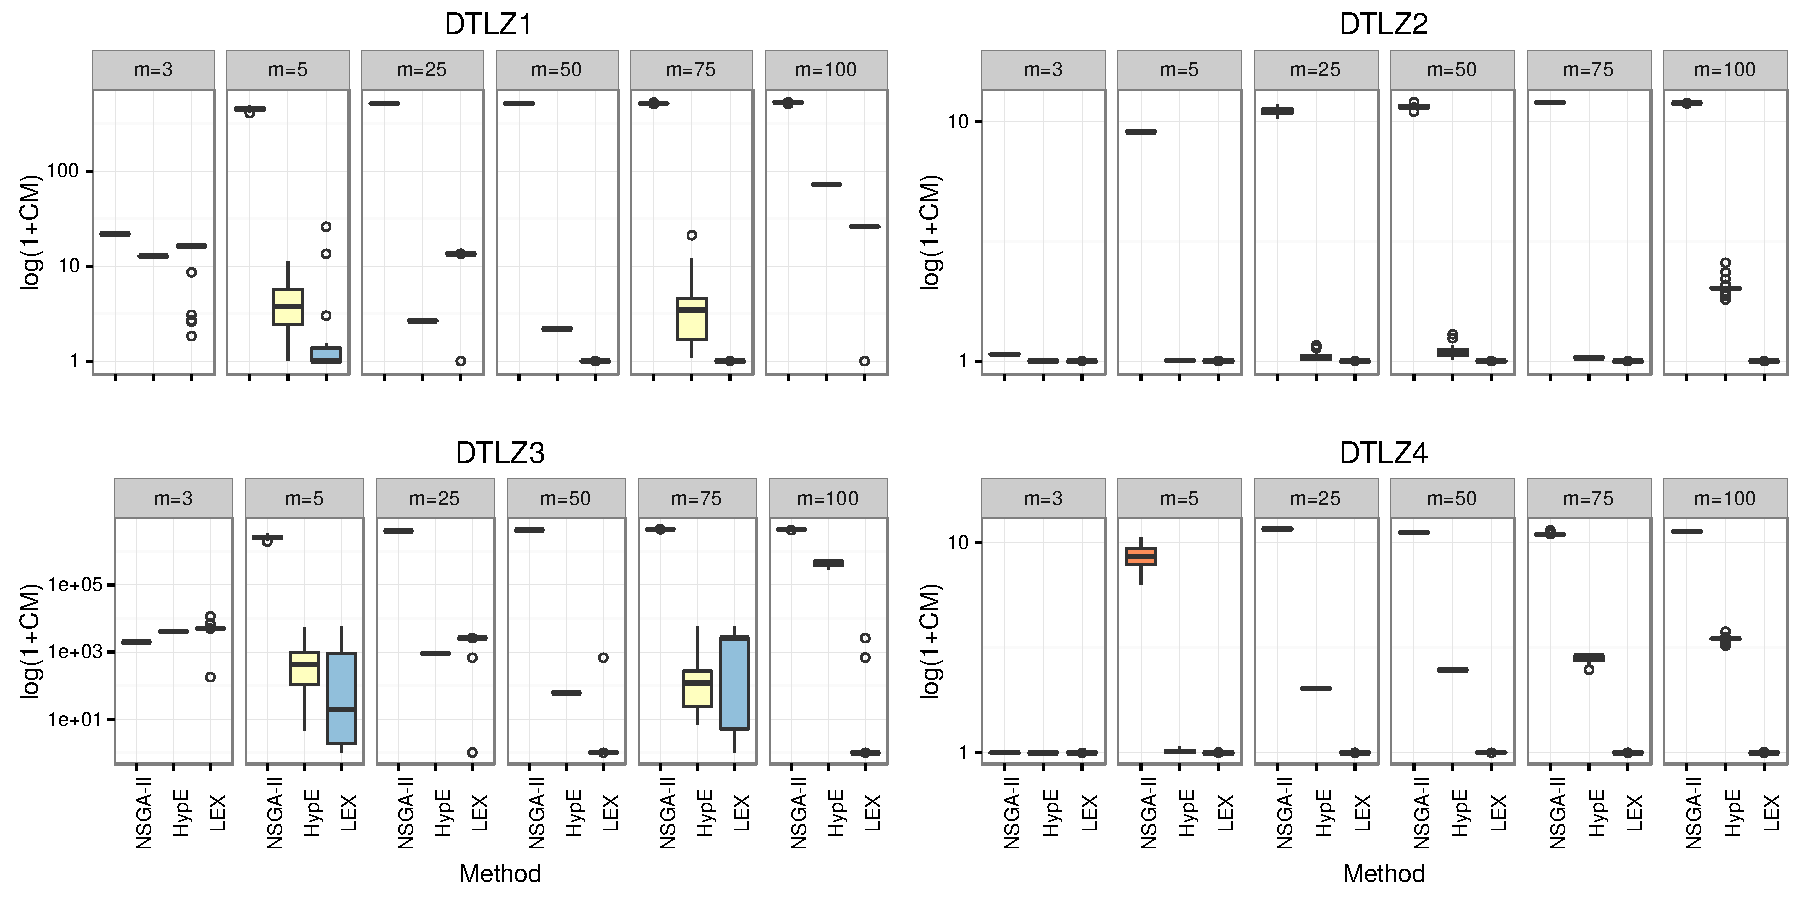
\includegraphics[width=\textwidth]{../analysis/figs/cm.pdf}
   \caption{Convergence Measure (CM) of the final populations of each selection method. Each
       quadrant is a DTLZ benchmark problem, and the columns corespond to the number of
    objectives.}\label{fig:cm}
\end{figure*}

\begin{figure*}
    \centering    
    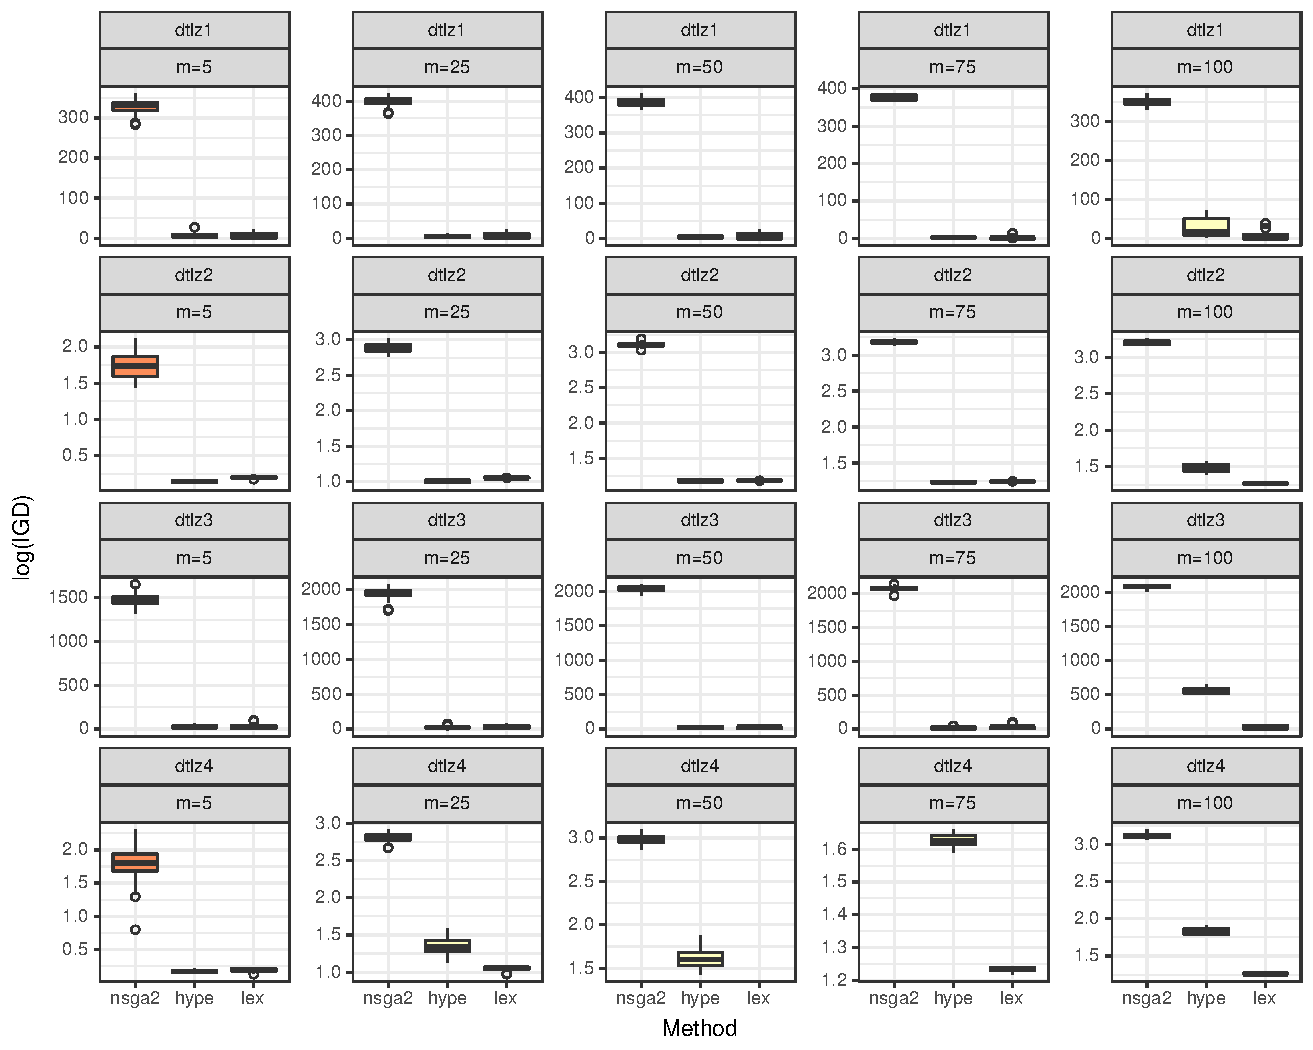
\includegraphics[width=\textwidth]{../analysis/figs/igd.pdf}
    \caption{Inverted Generational Distance (IGD) of the final populations of each selection method.
        Each quadrant is a DTLZ benchmark problem, and the columns corespond to the number of objectives.}\label{fig:igd}

\end{figure*}

\begin{figure}
    \centering
     \includegraphics[width=\columnwidth]{../analysis/figs/cm_rank.pdf}
   \caption{Average CM rankings of each algorithm as a function of $m$.}\label{fig:rcm}
\end{figure}

\begin{figure}
    \centering    
    \includegraphics[width=\columnwidth]{../analysis/figs/igd_rank.pdf}
    \caption{Average IGD rankings of each algorithm as a function of $m$.}\label{fig:rigd}
\end{figure}

\begin{figure}
    \centering    
    \includegraphics[width=\columnwidth]{../analysis/figs/timing.pdf}
    \caption{CPU time for each algorithm as a function of $m$.}\label{fig:time}
\end{figure}

\begin{table}[ht]
\centering
\caption{Significance test $p$-values comparing LEX to NSGA-II and HypE using the pair-wise Wilcoxon rank-sum test with Bonferroni correction. Bold indicates $p<$ 0.01.}
\label{tbl:wilcox}
\begingroup\footnotesize
\begin{tabular}{l l r r r r}
\toprule
&& \multicolumn{2}{c}{CM} & \multicolumn{2}{c}{IGD} \\Problem & m & NSGA-II & HypE & NSGA-II & HypE\\ 
 \midrule
&	3	&	\textbf{3.60e-13}&\textbf{2.32e-06}&\textbf{1.63e-07}&\textbf{2.32e-06}\\ 
&	5	&	\textbf{5.07e-17}&\textbf{1.29e-07}&\textbf{6.09e-16}&\textbf{1.63e-04}\\ 
&	25	&	\textbf{4.80e-13}&\textbf{1.90e-07}&\textbf{4.80e-13}&\textbf{1.90e-07}\\ 
DTLZ1&	50	&	\textbf{4.80e-13}&\textbf{4.80e-13}&\textbf{4.80e-13}&\textbf{4.80e-13}\\ 
&	75	&	\textbf{1.03e-11}&\textbf{1.96e-09}&\textbf{1.03e-11}&\textbf{2.57e-04}\\ 
&	100	&	\textbf{2.50e-12}&\textbf{6.22e-13}&\textbf{2.50e-12}&\textbf{2.74e-04}\\ 
\midrule 
&	3	&	\textbf{3.60e-13}&\textbf{3.60e-13}&\textbf{3.60e-13}&\textbf{3.60e-13}\\ 
&	5	&	\textbf{3.60e-13}&\textbf{3.60e-13}&\textbf{3.60e-13}&\textbf{3.60e-13}\\ 
&	25	&	\textbf{2.82e-11}&\textbf{2.82e-11}&\textbf{5.16e-12}&\textbf{5.16e-12}\\ 
DTLZ2&	50	&	\textbf{6.79e-11}&\textbf{6.79e-11}&\textbf{3.64e-12}&\textbf{3.64e-12}\\ 
&	75	&	\textbf{6.22e-13}&\textbf{6.22e-13}&\textbf{1.25e-13}&\textbf{1.25e-13}\\ 
&	100	&	\textbf{2.03e-12}&\textbf{1.81e-09}&\textbf{1.97e-12}&\textbf{2.66e-04}\\ 
\midrule 
&	3	&	\textbf{1.72e-11}&\textbf{1.72e-11}&\textbf{1.72e-11}&\textbf{1.72e-11}\\ 
&	5	&	\textbf{5.07e-17}&1.90e-01&\textbf{5.07e-17}&1.00e+00\\ 
&	25	&	\textbf{4.80e-13}&\textbf{2.65e-06}&\textbf{4.80e-13}&\textbf{1.72e-11}\\ 
DTLZ3&	50	&	\textbf{4.80e-13}&\textbf{4.86e-10}&\textbf{4.80e-13}&\textbf{4.86e-10}\\ 
&	75	&	\textbf{1.03e-11}&9.75e-02&\textbf{1.03e-11}&\textbf{8.03e-03}\\ 
&	100	&	\textbf{9.28e-13}&\textbf{1.49e-06}&\textbf{9.27e-13}&\textbf{1.49e-06}\\ 
\midrule 
&	3	&	\textbf{1.25e-13}&\textbf{5.30e-13}&\textbf{1.25e-13}&\textbf{5.30e-13}\\ 
&	5	&	\textbf{9.04e-11}&\textbf{7.04e-05}&\textbf{1.64e-10}&\textbf{2.09e-04}\\ 
&	25	&	\textbf{4.80e-13}&\textbf{4.80e-13}&\textbf{4.80e-13}&\textbf{1.72e-11}\\ 
DTLZ4&	50	&	\textbf{4.80e-13}&\textbf{4.80e-13}&\textbf{4.80e-13}&\textbf{4.80e-13}\\ 
&	75	&	\textbf{8.76e-12}&\textbf{3.18e-11}&\textbf{8.76e-12}&\textbf{3.18e-11}\\ 
&	100	&	\textbf{4.80e-13}&\textbf{6.14e-12}&\textbf{4.80e-13}&\textbf{6.14e-12}\\ 
\midrule 
\bottomrule
\end{tabular}
\endgroup
\end{table}
\label{tbl:wilcox}

\section{Discussion \& Conclusions}\label{s:con}

In this paper we adapt a selection method developed in the GP field to many-objective optimization. We were motivated to do so by recent recent theoretical results showing a relation between $\epsilon$-lexicase selection and Pareto-set boundary exploitation. Our analysis in \S\ref{s:methods} illustrates how $\epsilon$-lexicase performs selection in objective space and why such an approach may be useful as the number of objectives grow. 

The results of our experiment suggest that $\epsilon$-lexicase selection can performs very well on many-objective optimization problems. In comparison to NSGA-II and HypE, $\epsilon$-lexicase selection exhibits better convergence to the Pareto front, increasingly so for more objectives. Furthermore, for $m>3$, $\epsilon$-lexicase selection is able to preserve diversity among its solutions better than NSGA-II and in a similar manner to HypE, as measured by IGD. 

Future work should consider more adaptations of $\epsilon$-lexicase selection to incorporate concepts from other EMOs. For example, $\epsilon$-lexicase selection could be integrated with an archiving strategy as is common with other methods. We also intend to compare $\epsilon$-lexicase selection to other EMO algorithms, especially reference-point based methods, which are not considered in this study. In a broader sense, the success of $\epsilon$-lexicase selection suggests that it is useful to promote solutions near Pareto-set boundaries that perform well on randomized subsets of other objectives.

\section{Acknowledgments}
Omitted for review

\bibliographystyle{ACM-Reference-Format}
\bibliography{emo-lex} 

\end{document}
